\section{Amplificazione di chiralità}
\subsection{Chiralità in polimeri}\begin{frame}\frametitle{Chiralità in polimeri}
In polimeri con conformazione elicoidale si avranno {\bf regioni con rotazione destra o sinistra in equilibrio tra loro}; queste regioni saranno più lunghe se c'è alta energia di inversione. L'equilibrio può essere spostato con solventi chirali o chiralità sulle catene laterali.
\begin{columns}
\column{0.6\linewidth}In alcuni polimeri covalenti si ha una non-linearità dell'ellitticità con l'e.e. delle catene laterali. \cite{green}
\column{0.15\linewidth}\begin{figure}{\centering{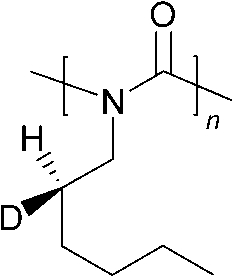
\includegraphics[width=1\textwidth]{sec1/polimero.png}}}\end{figure}\end{columns}\vspace{10pt}
\textbf{A differenza delle reazioni} in cui si ha amplificazione di chiralità qui \textbf{non aumenta l'e.e.} bensì aumenta la \textbf{chiralità osservabile}.

             \end{frame}
\subsection{Amplificazione di chiralità}
\subsubsection{Penalità nell'energia}\begin{frame}\frametitle{Amplificazione di chiralità}\framesubtitle{Penalità nell'energia}

I modelli utilizzati per l'amplificazione di chiralità considerano due contributi energetici:
\begin{itemize}
 \item penalità per {\bf inversione di elica}. \emph{Helix reversal penality: penalizes a helix reversal along the chain. It is invoked when two consecutive bonds have different conformations.}

 \item Penalità per {\bf errore puntuale}. \emph{Mismatch penality: penalizes a mismatch between the preferred screw sense of a monomer and the bonds near to it. It is used
whenever a “+” bond follows or precedes a “-” monomer, and vice versa. We apply the mismatch penalty twice when both monomers surrounding a bond are of the type incompatible with that bond.  }\cite{def}
\end{itemize}
\end{frame}
\subsubsection{Sergenti e soldati}\begin{frame}\frametitle{Amplificazione di chiralità}\framesubtitle{Sergenti e soldati}
Per valutare la non-linearità si possono misurare due effetti:

{\bf Sergenti e soldati}: tra molte unità monomeriche achirali poche unità chirali dirigono la chiralità della conformazione polimerica.

\begin{figure}{\centering{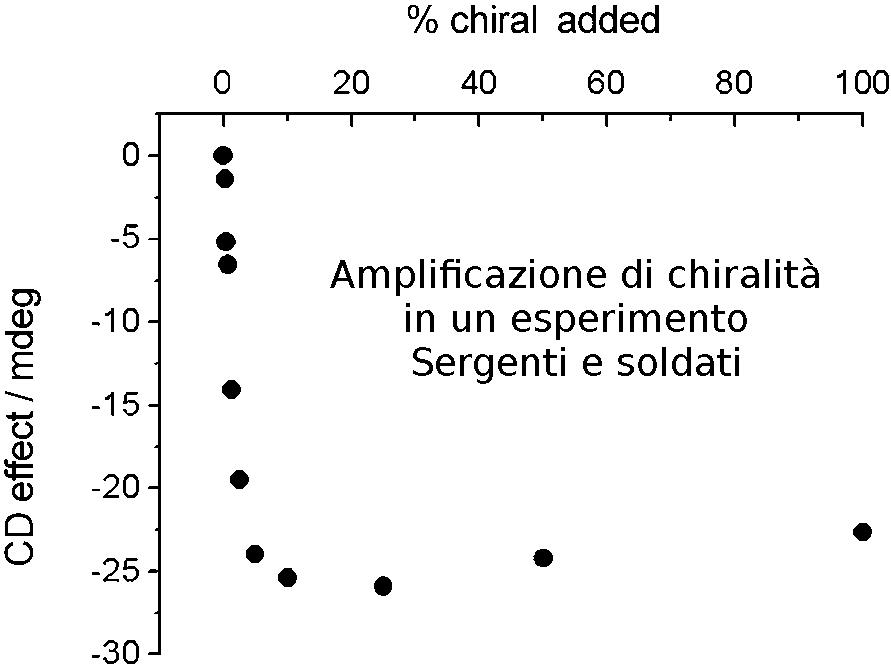
\includegraphics[width=0.5\textwidth]{sec1/sergenti.png}}}\end{figure}
\end{frame}

\subsubsection{Regola di maggioranza}\begin{frame}\frametitle{Amplificazione di chiralità}\framesubtitle{Regola di maggioranza}
{\bf Regola di maggioranza}: la conformazione di una catena con entrambi i monomeri enantiomerici viene dettata da quello in maggioranza. Avviene quando la penalità per errore puntuale 
 è inferiore alla penalità per inversione di elica.

\begin{figure}{\centering{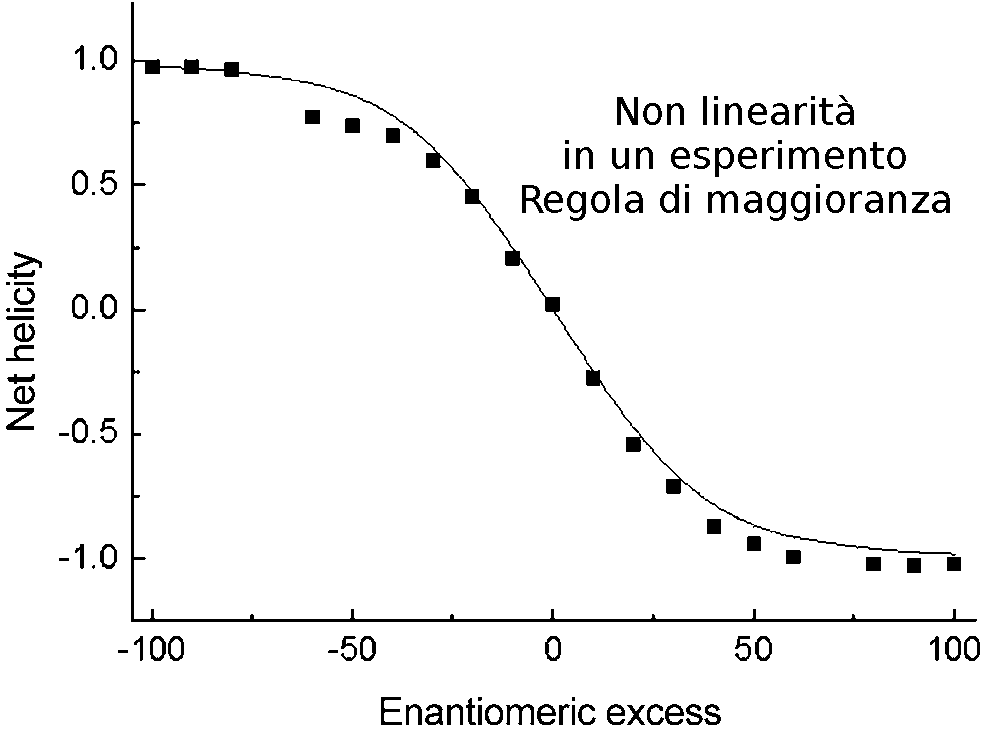
\includegraphics[width=0.4\textwidth]{sec1/maggioranza.png}}}\end{figure}
\end{frame}

